% Some commands used in this file
%\newcommand{\package}{\emph}

\chapter{Mobile Robot Application Development}
\label{chap:app dev}
It is needed to have a software basis for ITU-AGVs that will be used to develop specific applications for various tasks in the future possible projects, theses and works. ITU-AGVs have built before ROS was developed. At the time when ITU-AGVs built, the software systems that used were different and custom so the software of the robots was written concerning them which became out-of-date now.
\par 
As mentioned previously in the Introduction chapter, the goal is to construct a set of applications for the basic problems and needs using up-to-date tools. It is desired to write the embedded code for LLPL so the robots can be communicate with ROS and to develop ROS applications for tele-operation, sensor integration and reading, odometry estimation, data collection and offline map building. With realization of this basis, ITU-AGVs can be used as multi-purpose indoor land vehicle kits available using rapidly for educational purposes, theses, autonomous system design and algorithm development at ITU Robotics Laboratory.
\par
The processing work is divided with a hierarchy. Low Level Processing Layer (LLPL) is responsible for getting commands, communicating motor drivers to drive the motors as desired in the given commands, requesting encoder values and sending them to High Level Processing Layer. High Level Processing Layer is responsible for complex calculations and is the part where the ROS runs. The signal chart of ITU-AGVs can be seen in Figure ~\ref{fig:agvSignal}. The project is started with LLPL work and then HLPL after. 

\begin{figure}[h]
	\centering
	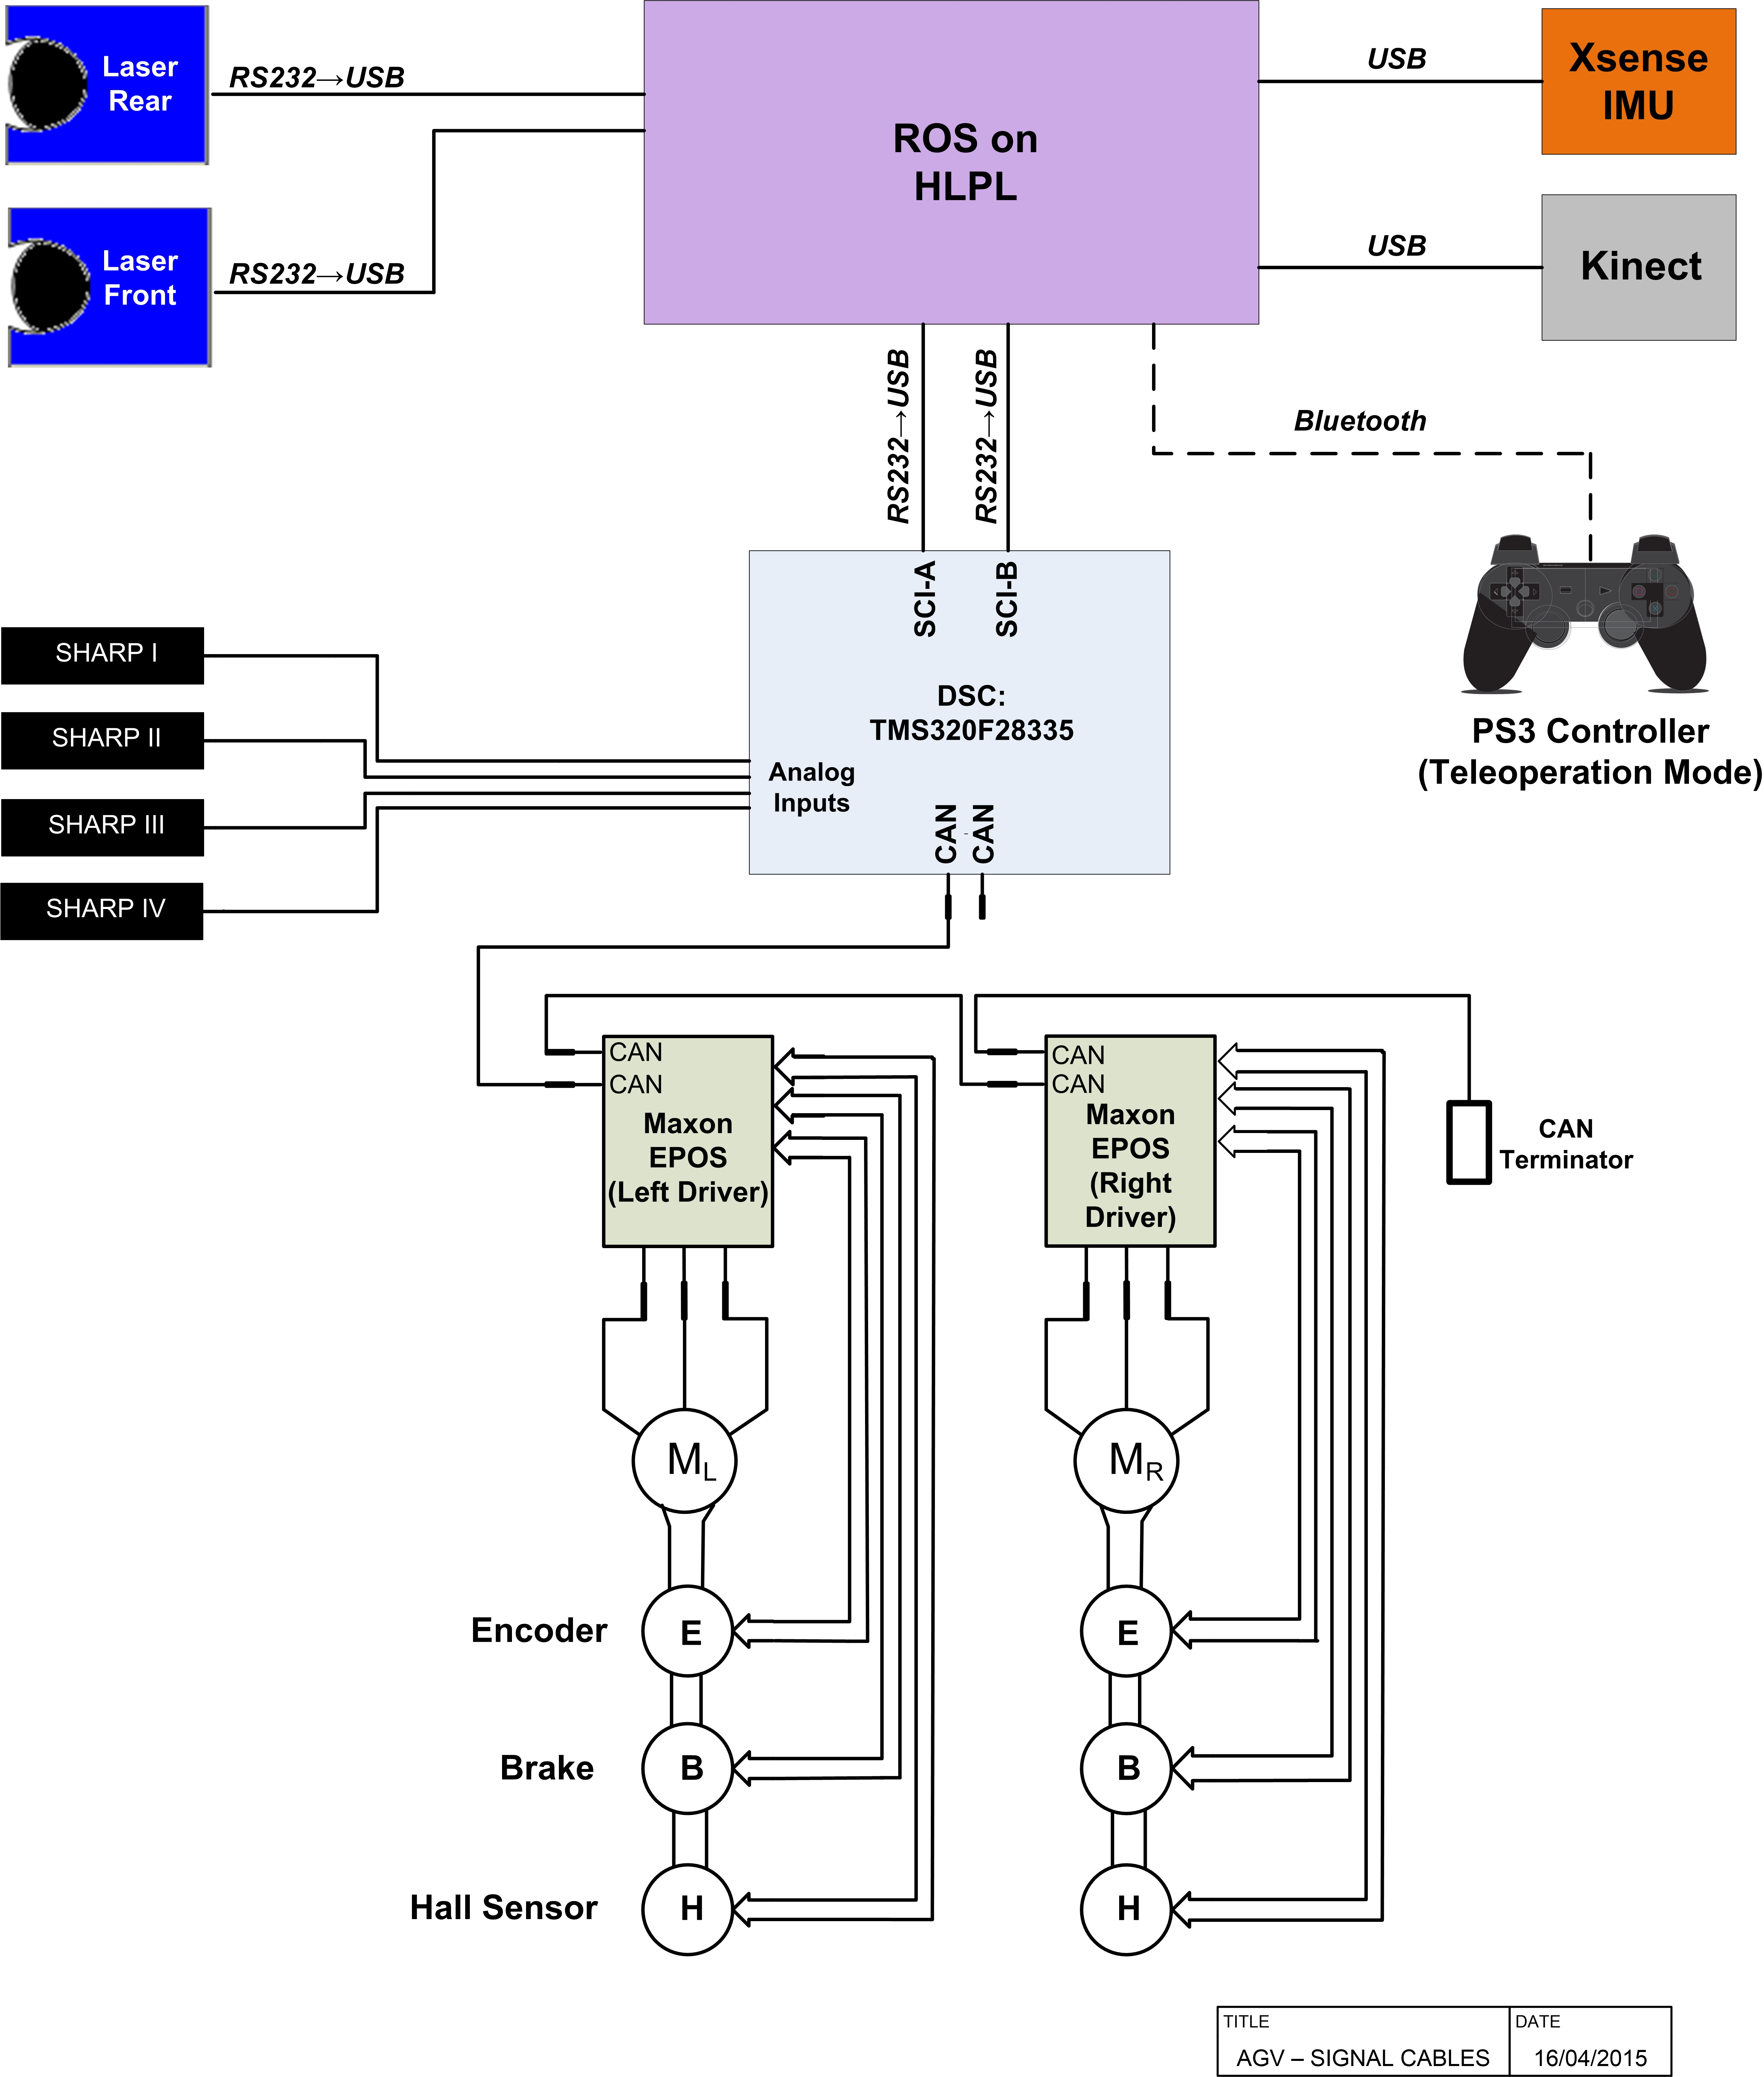
\includegraphics[scale=0.45]{images/agvSignal}
	\caption{Signal chart of ITU-AGVs}
	\label{fig:agvSignal}
\end{figure}

\section{Embedded Program Development for LLPL}
\label{sec:embedded dev}
The embedded software for TMS320F28335 microcontrollers at LLPL is developed using Simulink Embedded Target Coder in MATLAB r2012b and then the make files are uploaded to the microcontroller using TI Code Composer Studio v4. 
	\subsection{Communication with EPOS Drivers}
	\label{subsec:comm with epos}
	The Maxon EPOS 70/10 motor drivers are designed to be used with CANOpen protocol. In CAN communication several hardware are connected as slaves to a master using a CAN Bus. The communication and configuration occurs with using array of variables called objects. Object dictionary includes all object addresses with 16-bit index and 8-bit sub index. 
	\par
	EPOS drivers have their configurable controllers and there are several driving modes such as position mode, velocity mode, profile velocity mode and so on. It is desired to send velocity commands to the LLPL and to settle the motors on the desired velocity references. So the operation mode would be selected as the profile velocity mode. 
	\par
	According to the EPOS 70/10 Manual~\cite{eposManual}, the motors are controlled with given profile velocity and acceleration limits and selection of motion profile type. Motion profile type can be selected as linear or sinusoidal. It is desired to obtain a sinusoidal profile. In the manual, all configuration and communication object values and their places in the work flow are provided. 
	\par
	\begin{figure}[h]
		\centering
		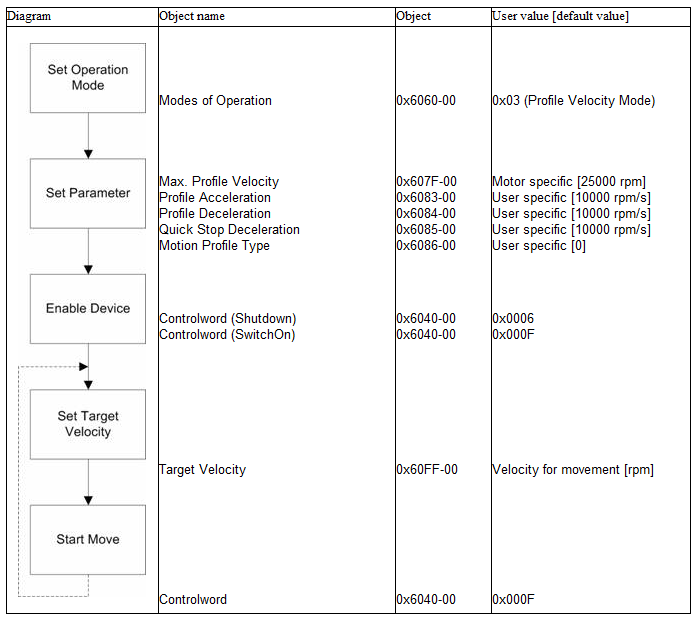
\includegraphics[scale=0.7]{images/eposProfileVelocity}
		\caption{Configuration flow chart for profile velocity mode ~\cite{eposManual}}
		\label{fig:eposProfileVelocity}
	\end{figure}
	In Simulink, a state chart diagram is created in order to make the program flow as a state machine. In the program, according to the EPOS 70/10 Manual the necessary configurations are being made. First, all CANOpen nodes are being reset and all slaves are being set as operational. Then according to the chart in Figure ~\ref{fig:eposProfileVelocity}, the operation mode is being selected as profile velocity mode, the values for maximum profile velocity, profile acceleration, profile deceleration, quick stop deceleration and motion profile type are being configured over their objects and a necessary reset is being done. After these configurations, the program enters a loop. In the loop, the commands are being taken from HLPL over SCI-A (Serial Communication Interface - A) serially. The commands are being parsed and left and right motor commands are separated and set as target velocity values. The control word is being sent and encoder values are being requested. After the encoder values are received, they are being sent to HLPL over SCI-B and the loop begins again. The flow of the state chart diagram in Simulink can be seen in Figure ~\ref{fig:simulinkStateFlow}.
	\begin{figure}
		\centering
		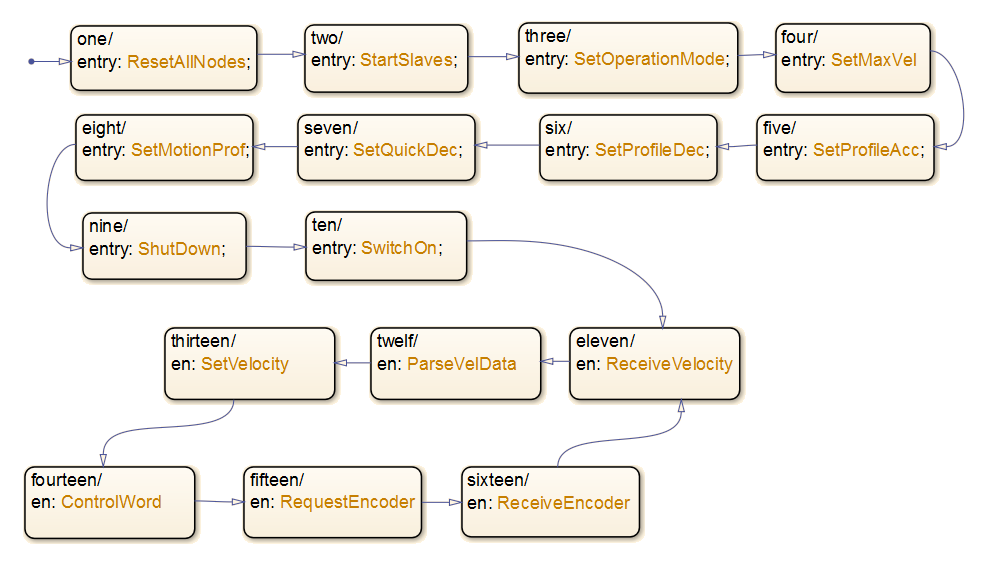
\includegraphics[scale=0.5]{images/simulinkStateFlow}
		\caption{State chart flow diagram of LLPL in Simulink}
		\label{fig:simulinkStateFlow}
	\end{figure}
	
	\subsection{Communication with HLPL}
	\label{subsec:comm with hlpl}
	The velocity commands are designed to be in one sixteenth of desired rpm values at the motor shaft before gear-box. LLPL takes commands in 16-bit integers. The command word will be sent starting with “\#” character and ending with “!” character. The first 16-bits after starting character will be the left motor command and the second 16-bits until the end character will be the right motor command. Commands are 16-bits and the first byte of each command is for direction and the second byte is for one sixteenth of the rpm value desired at the motor shaft before the gear-box. Before sending the values to the drivers, this value is multiplied by. It is important to remind the gear-box on the motor since it reduces the rpm with a ratio of 1:100. 
	\par
	For example, if it is wanted to drive the wheels at 40 rpm, a basic calculation can be made. The rpm value at the shaft of the motor before the gear-box would be $40\times100=4000$. This is the target rpm value, so the second byte of the command must have the value of $4000\div16=250$. 
	\par
	The direction is set such that, if the value of the direction byte is less than or equal to 127 it is counted as positive direction and the otherwise is negative direction. So the necessary word needed to be send to LLPL in order to drive wheels at 40 rpm in the positive direction should be 
	$[\#\text{0 250 0 250}!]$. The parsing is made in then made in LLPL. 
	\par
	EPOS 70/10 can provide various calculations with encoder values and it can give position and velocity. The encoder values are being sent in 16-bits to HLPL. Both SCI-A and SCI-B serial communications are set at 115200 baud.
		
	\subsection{Testing the LLPL}
	\label{subsec:testing llpl}
	In order to test the embedded software and the serial communication a simple test script is written with Python. In the script the direction and desired wheel rpm values are requested from the user for left and right wheels and the command word is calculated and sent over serial port to the ITU-AGVs (Figure ~\ref{fig:testScript}). After using this test script, it is concluded that the LLPL is functionally working and the project can be moved on to HLPL.
	
	\begin{figure}[h]
		\centering
		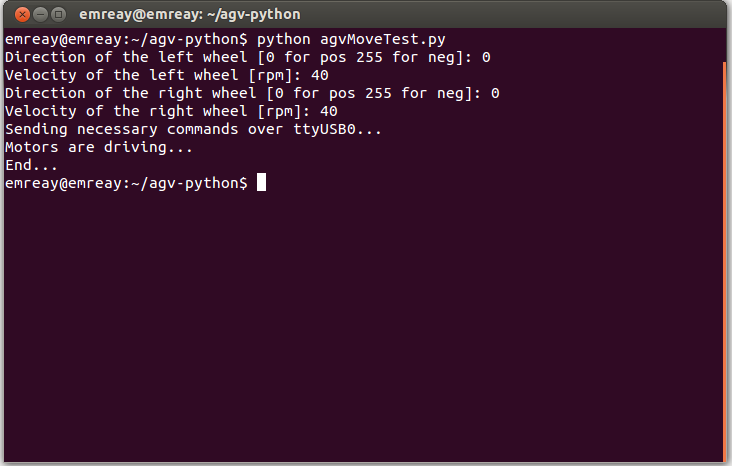
\includegraphics[scale=0.65]{images/testScript}
		\caption{Testing LLPL with a written Python script}
		\label{fig:testScript}
	\end{figure}
	
\section{ROS Programming for HLPL}
\label{sec:programming for hlpl}

	\subsection{ROS Installation \& System Initialize}
	\label{subsec:ros install and init}
	Pre-compiled repositories for ROS distributions are officially supported and supplied for Ubuntu. The HLPL would be ROS running on Ubuntu 12.04 LTS on a notebook computer. ROS Groovy distribution is supported on Ubuntu 12.04 LTS so its complete packages are installed according to the directives at ROS Wiki Website. 
	\par
	After installation a workspace is needed to be created. Workspace is the container folder where all the packages and their relative files are stored. Catkin build system has a command to easily create a workspace for ROS. 
	\par
	There are several packages needed to be installed that are not included in the ROS core packages. These are usually specific work or hardware packages. Since the sensors to be installed are decided, their relative software driver packages for ROS are installed including ps3joy for Play Station 3 joystick, sicktoolbox wrapper for laser sensors and xsens driver for IMU. 
	\par
	To contain the applications that are going to be written, a ros package is needed to be created. Catkin also provides an easy package creation with a command and its several arguments. Packages usually depend on other packages in order to use their functionalities. So a package named \textit{agv} is created with dependencies to \textit{roscpp} and \textit{rospy} packages. This package together with all the written ROS codes in this project is available at the link given in Appendix ~\ref{appendix}.
	\subsection{Teleoperation Application}
	\label{subsec:teleop app}
	Teleoperation is a vital functionality for manual data collection or to move the robot to the application areas. It is needed to be able to move ITU-AGVs manually as desired in order to collect laser data or images for use in algorithm development on Simultaneous Localization and Mapping (SLAM), loop closure or similar applications. 
		\subsubsection{Simulation}
		\label{subsec:simulation}
		Before directly passing to work on ITU-AGVs, the teleoperation is desired to be applied on a simulation environment of ROS. To achieve this, a visual model has to be created. Rviz visualization environment supports an xml based format for basic 3D robot representation called Unified Robot Description Format (*.urdf). It is a simple parser with a simple syntax. So basically, a box with to wheels in the dimensions and placement of the ITU-AGVs can be created by a urdf file as follows;
		\lstinputlisting[title={Urdf code for ITU-AGVs}]{codes/agv_.urdf}
		So basically the links and joints are geometrically defined with their positions, dimensions together with their relationship with each other. So their hierarchy tree can be understood by the system and it is possible to visually see the tree as in Figure ~\ref{fig:urdfTree}. When the created urdf file is opened in Rviz, a simple box and two wheels with the given parameters can be seen as in Figure ~\ref{fig:agv-urdf}. This visualization is a simple and quick solution. But it is possible to integrate more realistic 3D models. Rviz supports Collada file format (*.dae) which is an open xml schema, so the 3D models created in various CAD software such as Google SketchUp can be converted to Collada file and implemented to Rviz~\cite{Martinez-Ros}. So a 3D model of ITU-AGVs are created using Google SketchUp and it is converted to the Collada file (Figure ~\ref{fig:agv-dae}).
		\begin{figure}[h]
			\centering
			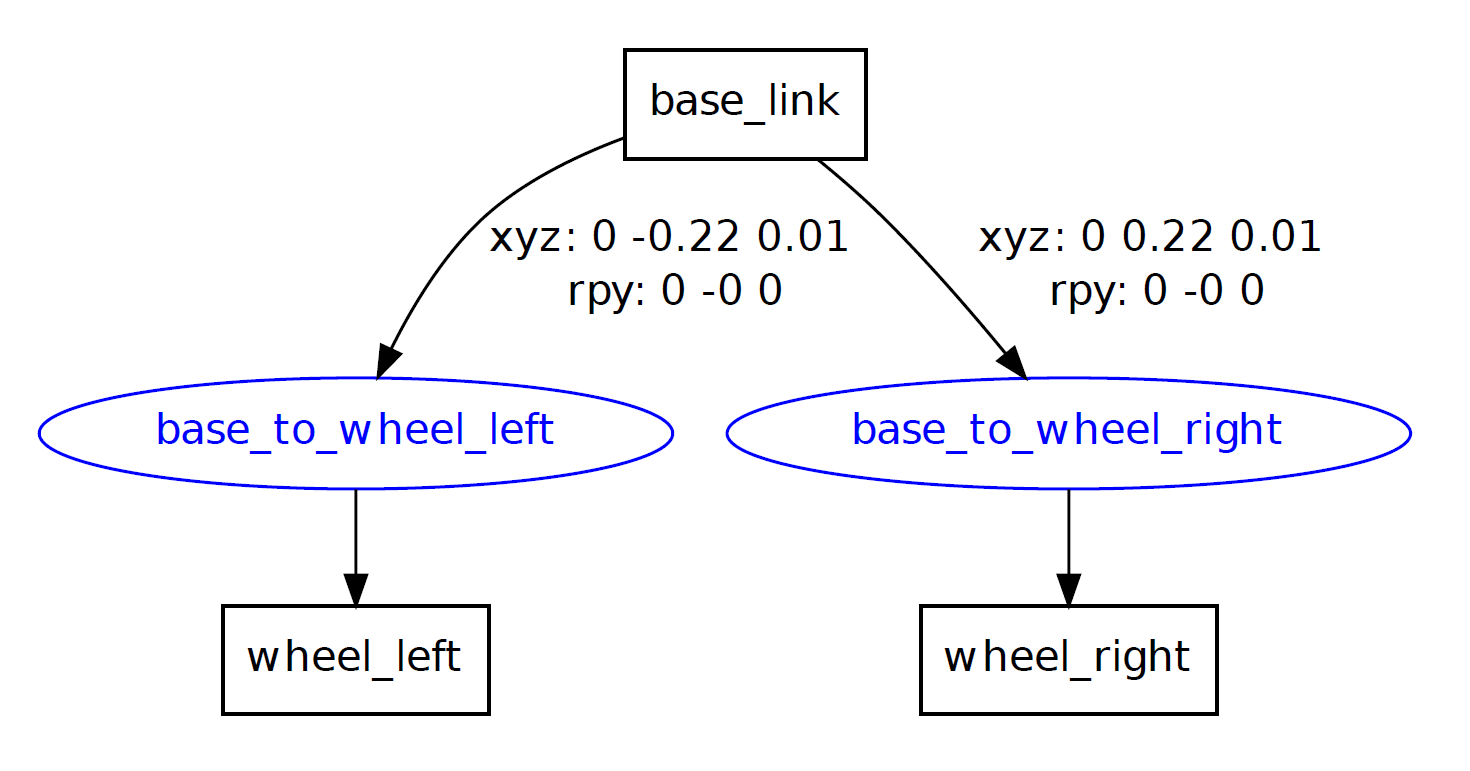
\includegraphics[scale=0.3]{images/urdfTree}
			\caption{Urdf tree}
			\label{fig:urdfTree}
		\end{figure}
		
		\begin{figure}[h]
			\centering
			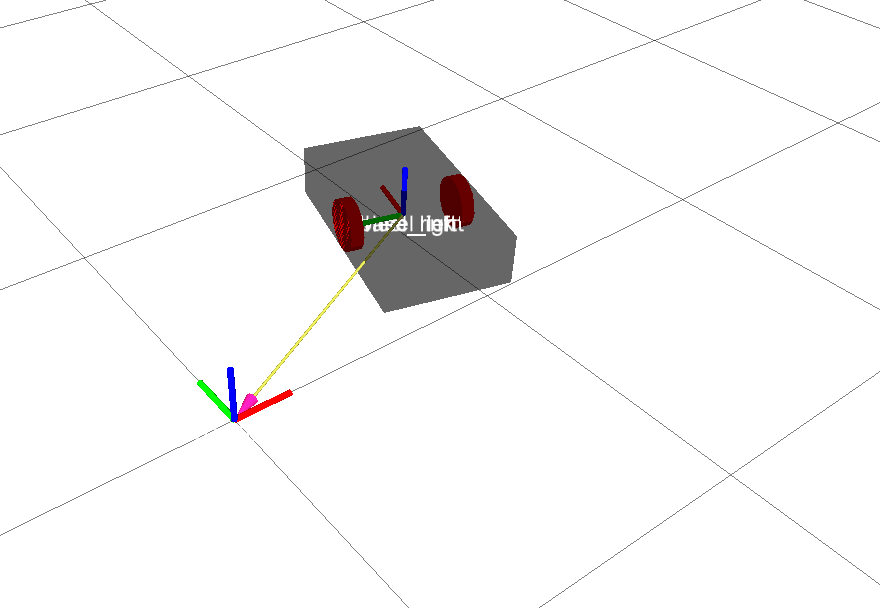
\includegraphics[scale=0.55]{images/agv-urdf}
			\caption{Urdf model of ITU-AGVs}
			\label{fig:agv-urdf}
		\end{figure}
		\par
		It is wanted to realize the tele-operation using the Play Station 3 joystick. It is desired to control with both analog buttons and digital buttons. In the analog mode, the vertical values of left and right analog buttons will be the angular velocity references (in rpm) of left and right wheels. In digital mode, cross buttons will drive the motors on constant angular velocities. The up and down direction buttons will move the robot forwards and backwards, left and right buttons will drive the motors in the opposite directions resulting in a clockwise and a counter clockwise rotation around the central point. Lastly it is desired to only one mode at a time, hence while R2 button on the joystick is pushed digital mode would be active and otherwise analog mode would be active. 
		\par
		\begin{figure}[h]
			\centering
			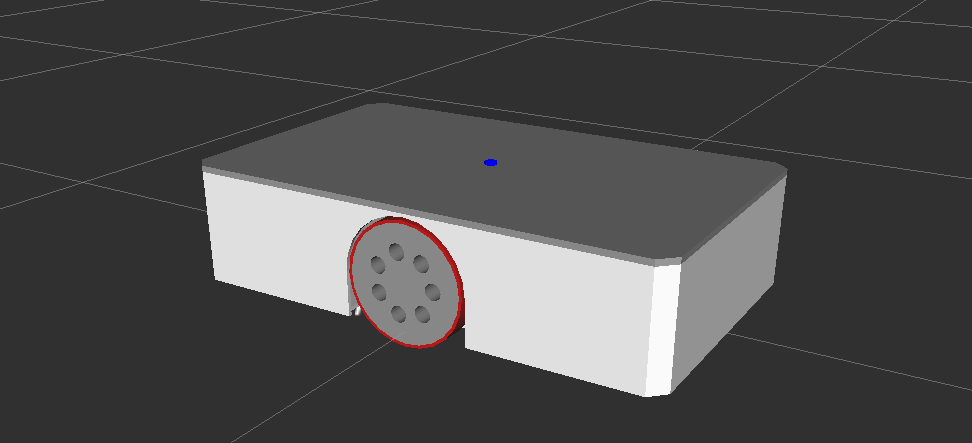
\includegraphics[scale=0.5]{images/agv-dae}
			\caption{3D model ITU-AGVs opened in Rviz}
			\label{fig:agv-dae}
		\end{figure}		
		Using the installed ps3joy package, communication with PS3 joystick over Bluetooth is handled and the button values are published to ROS environment. A node that subscribed to the joystick topic is created. This node gets the joystick button values, and passes the values of the necessary buttons as the relevant joint’s velocity with multiplying it with a scalar, then publishes all the joint states. Another node is written so that it is subscribed to the topic that joint states are published. When the joint states data is received this node passes the velocity data to the parameter server in the callback function. Then in the main loop, it calculates the odometry of the robot and publishes the odometry information. 
		\par
		After building the nodes and launching them the 3D model of ITU-AGVs have successfully moved with using the PS3 joystick (Figure ~\ref{fig:agv-teleop-sim})	
		\begin{figure}[h]
			\centering
			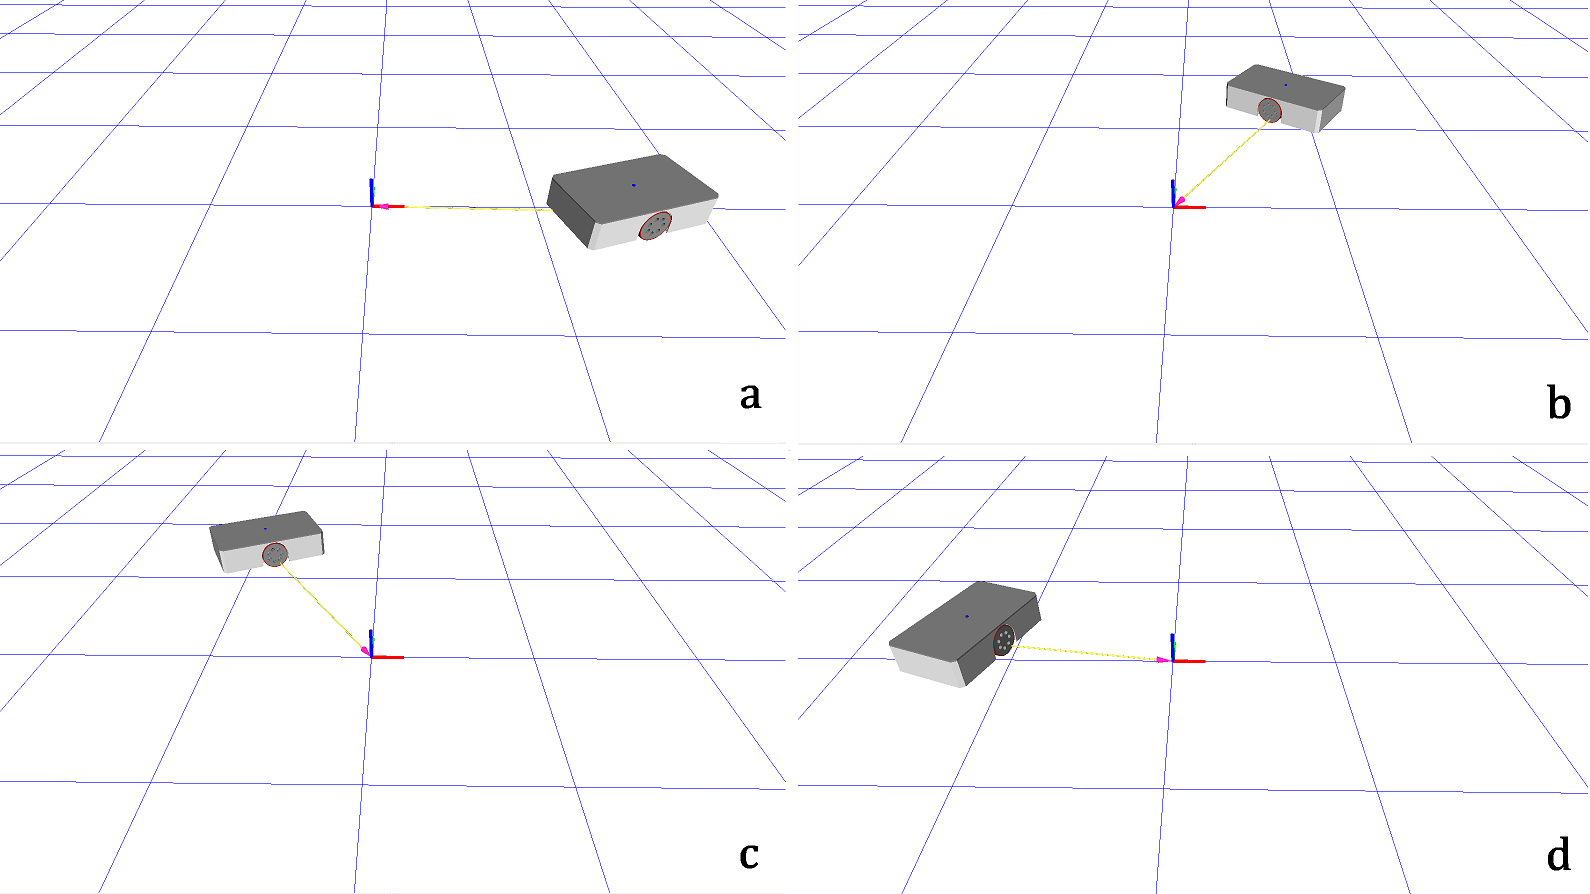
\includegraphics[scale=0.3]{images/agv-teleop-sim}
			\caption{Teleoperation of ITU-AGV model in Rviz}
			\label{fig:agv-teleop-sim}
		\end{figure}		
		\subsubsection{Teleoperation of ITU-AGVs}
		\label{subsec:teleop pkg}
		Since the teleoperation is successfully made on the simulation, it is convenient to realize the teleoperation of ITU-AGVs. A similar but modified approach is made. A node is created so that it would subscribe to the joystick topic and every time the joystick data is received it takes the needed button values. If the R2 button is pressed, it configures several variables depending on the values of digital cross buttons. If R2 button is not pressed, it configures the same variables depending on the analog button values. In the main loop, the node publishes an array of the variables which are configured in the callback function. This array is in the form that has been specified in Section ~\ref{subsec:comm with hlpl}. In order to send the commands to ITU-AGVs, another node is subscribed to the topic in which the array is published and it sends the array to LLPL of ITU-AGVs over a serial COM port. After the nodes are built, teleoperation of ITU-AGVs is successfully achieved. Node graph is shown for the teleoperation in Figure ~\ref{fig:teleop-graph}. It is possible to see the node graph in ROS in order to examine the relationships of nodes over topics and to see which nodes and topics are active. This is a powerful feature for diagnostics. 
		\begin{figure}[h]
			\centering
			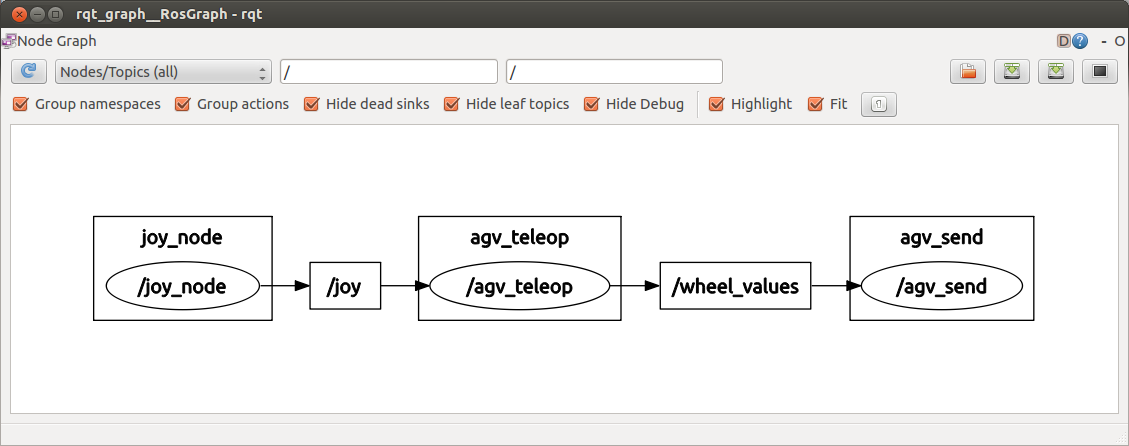
\includegraphics[scale=0.43]{images/teleop-graph}
			\caption{Node graph (rqt-graph) of teleoperation}
			\label{fig:teleop-graph}
		\end{figure}
	\subsection{Sensor Integration}
	\label{subsec:sensor integration}
	Software packages of various sensors were installed during the system initialize. Since the teleoperation is applicable, reading stable data from the sensors on ROS is the next goal. 
		\begin{figure}[h]
			\centering
			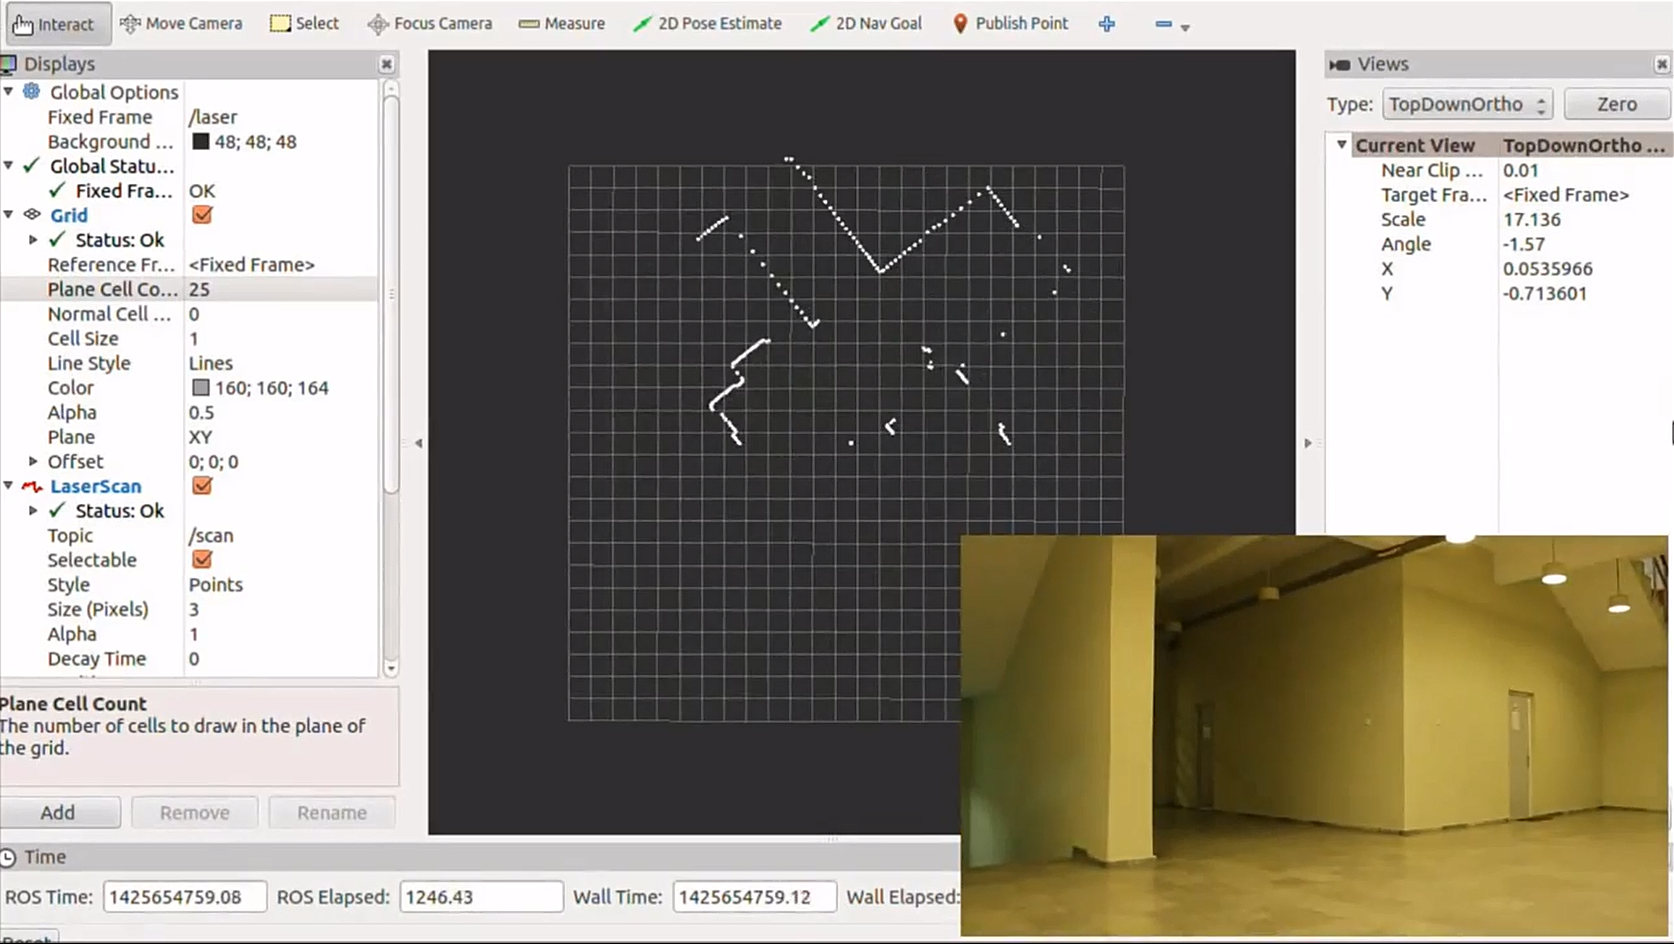
\includegraphics[scale=0.3]{images/lidar-sim}
			\caption{Simultanoues stream of LIDAR data on Rviz and the image of real environment}
			\label{fig:lidar-sim}
		\end{figure} 
		\subsubsection{Encoder Reading}
		\label{subsec:encoder reading}
		The encoder values are sending over SCI-B as they have configured to do in Section ~\ref{subsec:comm with hlpl}. In the HLPL, they have to be read. To read the encoder values, a Python node is written. In this node, the COM port assigned to SCI-B (ttyUSB1) is continuously listened. Since the sending format is the same (start character as “\#”, end character “!”), the node converts the unsigned 16-bit integer values to signed 16-bit values and publishes the converted values on a topic. 
		\subsubsection{IMU Reading}
		\label{subsec:imu reading}		
		The related ROS package for Xsens MTi IMU was installed before. Using this package a launch file is created and the node that publishes IMU data is successfully initialized. In order to calibrate the data and make certain settings the software provided by Xsens is used. As shown in Figure ~\ref{fig:xsens-test}, the robot is rotated around its center for approximately 90 $^{\circ}$ clockwise and counter clockwise and the yaw angle is plotted from the IMU data. It can be also seen that the robot settles smoothly in sinusoidal profile as the motor drivers are configured to do in Section ~\ref{subsec:comm with epos}.
		\begin{figure}[h]
			\centering
			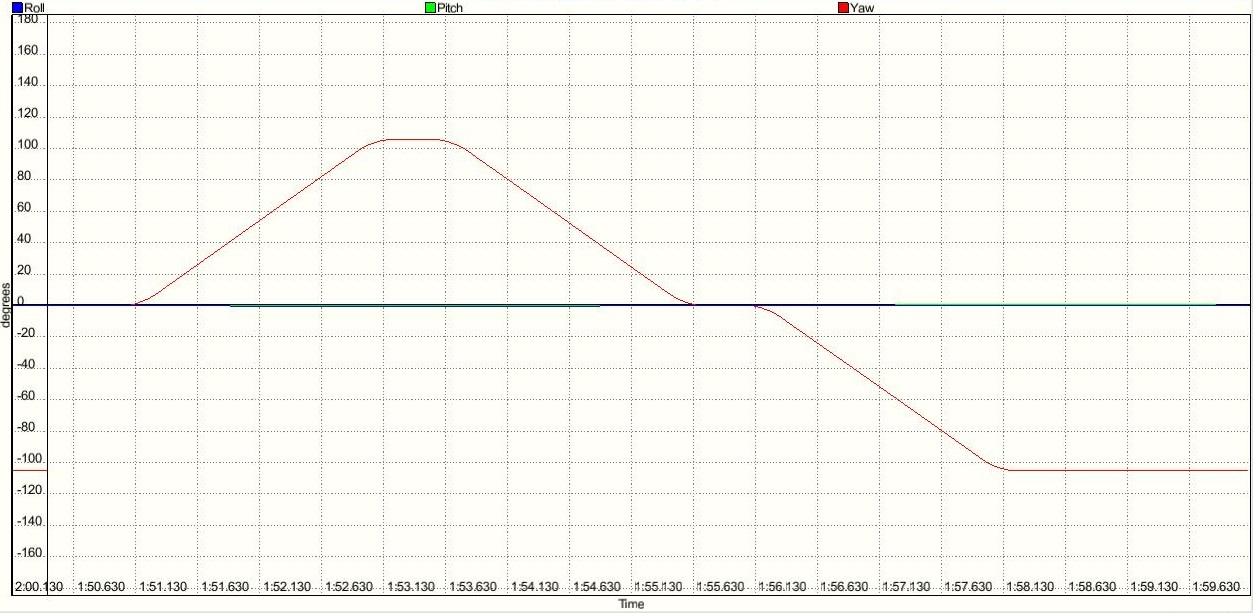
\includegraphics[scale=0.4]{images/xsens-test}
			\caption{Yaw angle values is retrieved from IMU while the robot is rotating}
			\label{fig:xsens-test}
		\end{figure} 	
		\subsubsection{LIDAR Reading}
		\label{subsec:lidar reading}	
		The related package publishes laser scan data on ROS environment. A launch file is created and the data scanned by the LIDAR is simultaneously published on Rviz as in the Figure ~\ref{fig:lidar-sim}.	
		\subsubsection{Kinect Reading}
		\label{subsec:kinect reading}		
		OpenNI driver packages for Kinect are installed. After a launch file is created, both RGB and point cloud data are streamed to Rviz (Figure ~\ref{fig:kinect-pcl}).
		
	\subsection{Odometry Estimation}
	\label{subsec:odom estimation}
	Odometry estimation is a vital step since it is not possible to robot to autonomously move, navigate and plan without the information of its position and orientation with respect to the environment. The basic odometry calculation is made using the left and right wheel velocities obtained from the motor encoders. However, this calculation alone might give inexact or wrong odometry information due to errors in the calculation of velocity or slippage of the robot wheels.
		\begin{figure}[h]
			\centering
			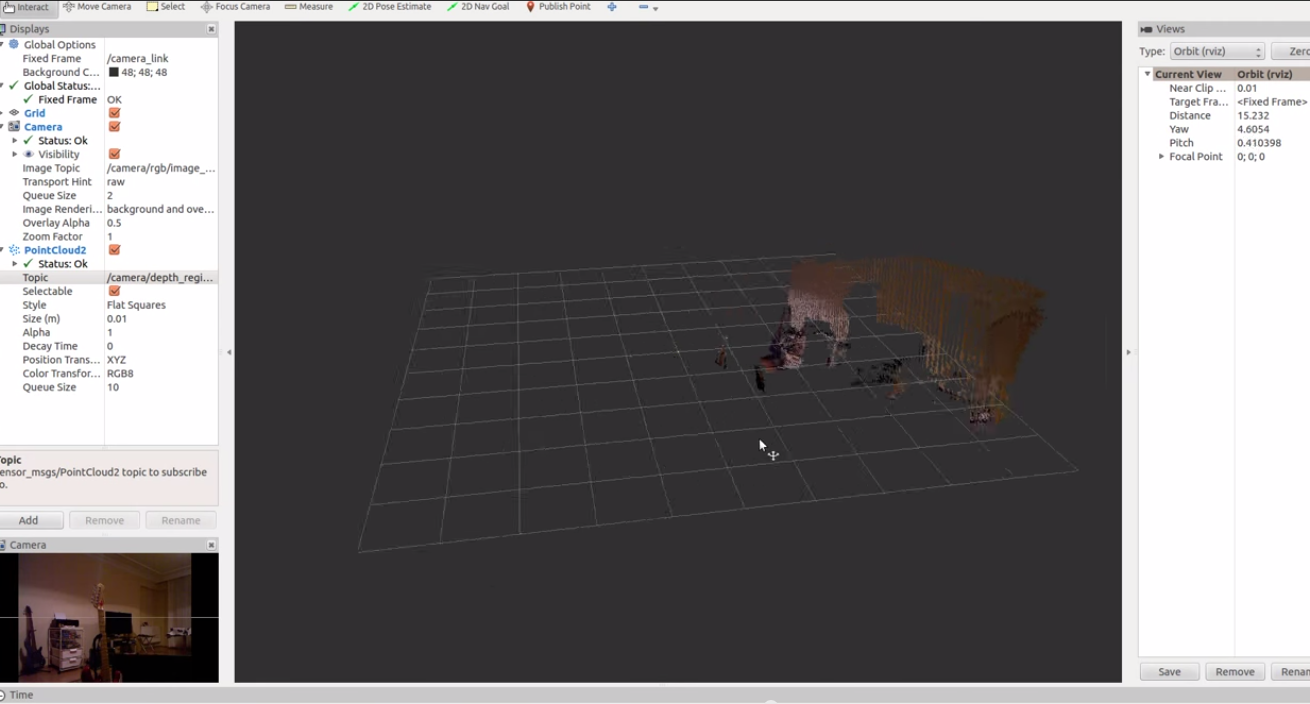
\includegraphics[scale=0.38]{images/kinect-pcl}
			\caption{RGB and point cloud data stream from Kinect on Rviz}
			\label{fig:kinect-pcl}
		\end{figure}	
	\par
	To get better and more reliable odometry information, the present-day robotics systems use IMU data or vision along with the encoders. The process called data fusion is applied in these cases to integrate various data. There are various advanced methods for multi-sensor data fusion which are beyond the scope of this project. However, there is a ROS package that provides data fusion for IMU and encoder data to estimate the pose of a robot using Extended Kalman Filter (EKF) named robot pose ekf  ~\cite{robotPoseEkf}. 
	\par
	Extended Kalman Filter in this case estimates an optimal value for odometry from the data of IMU and encoder and with a covariance matrix that tells how much accurate the data are. Using robot pose ekf package, the fused odometry information can be obtained. The necessary launch file is created so the nodes that publish IMU data and encoder values are started and the fused odometry information is published on a topic. The node graph can be seen in Figure ~\ref{fig:ekf-graph}.

	\begin{figure}
		\centering
		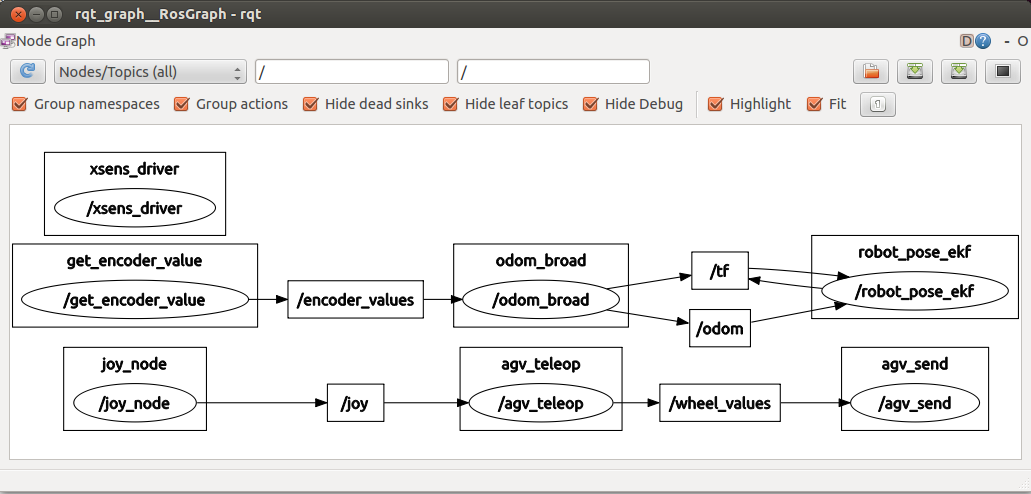
\includegraphics[scale=0.42]{images/ekf-graph}
		\caption{Node graph (rqt graph) while the robot pose ekf is publishing fused odometry data}
		\label{fig:ekf-graph}
	\end{figure}
				 
	\subsection{Offline Map Building}
	\label{subsec:offline mapping}					
	It is desired to build maps using collected data from the indoor environment. ROS can record and replay messages with makes it suitable for data collection. Since the odometry of ITU-AGVs can be estimated, sensors are installed, working and ready to publish data on ROS environment it is now possible to collect the necessary data while moving the ITU-AGVs to the desired areas. 
	\par
	A launch file for activating the nodes for IMU and encoder reading, odometry calculations and laser reading is created. 
	ROS records data to bag files and it is very simple to record desired or all topics that are active at the time of record. In this case the laser data and fused odometry information is needed to build a map. One of the ITU-AGVs is moved using Play Station 3 joystick while the selected topics are recorded inside ITU Electric and Electronics Faculty. After the data collection is done, the recorded data is replayed and using another package called gmapping an offline map of Control and Automation Department corridor is built as shown in Figure ~\ref{fig:map}.
	\begin{figure}
		\centering
		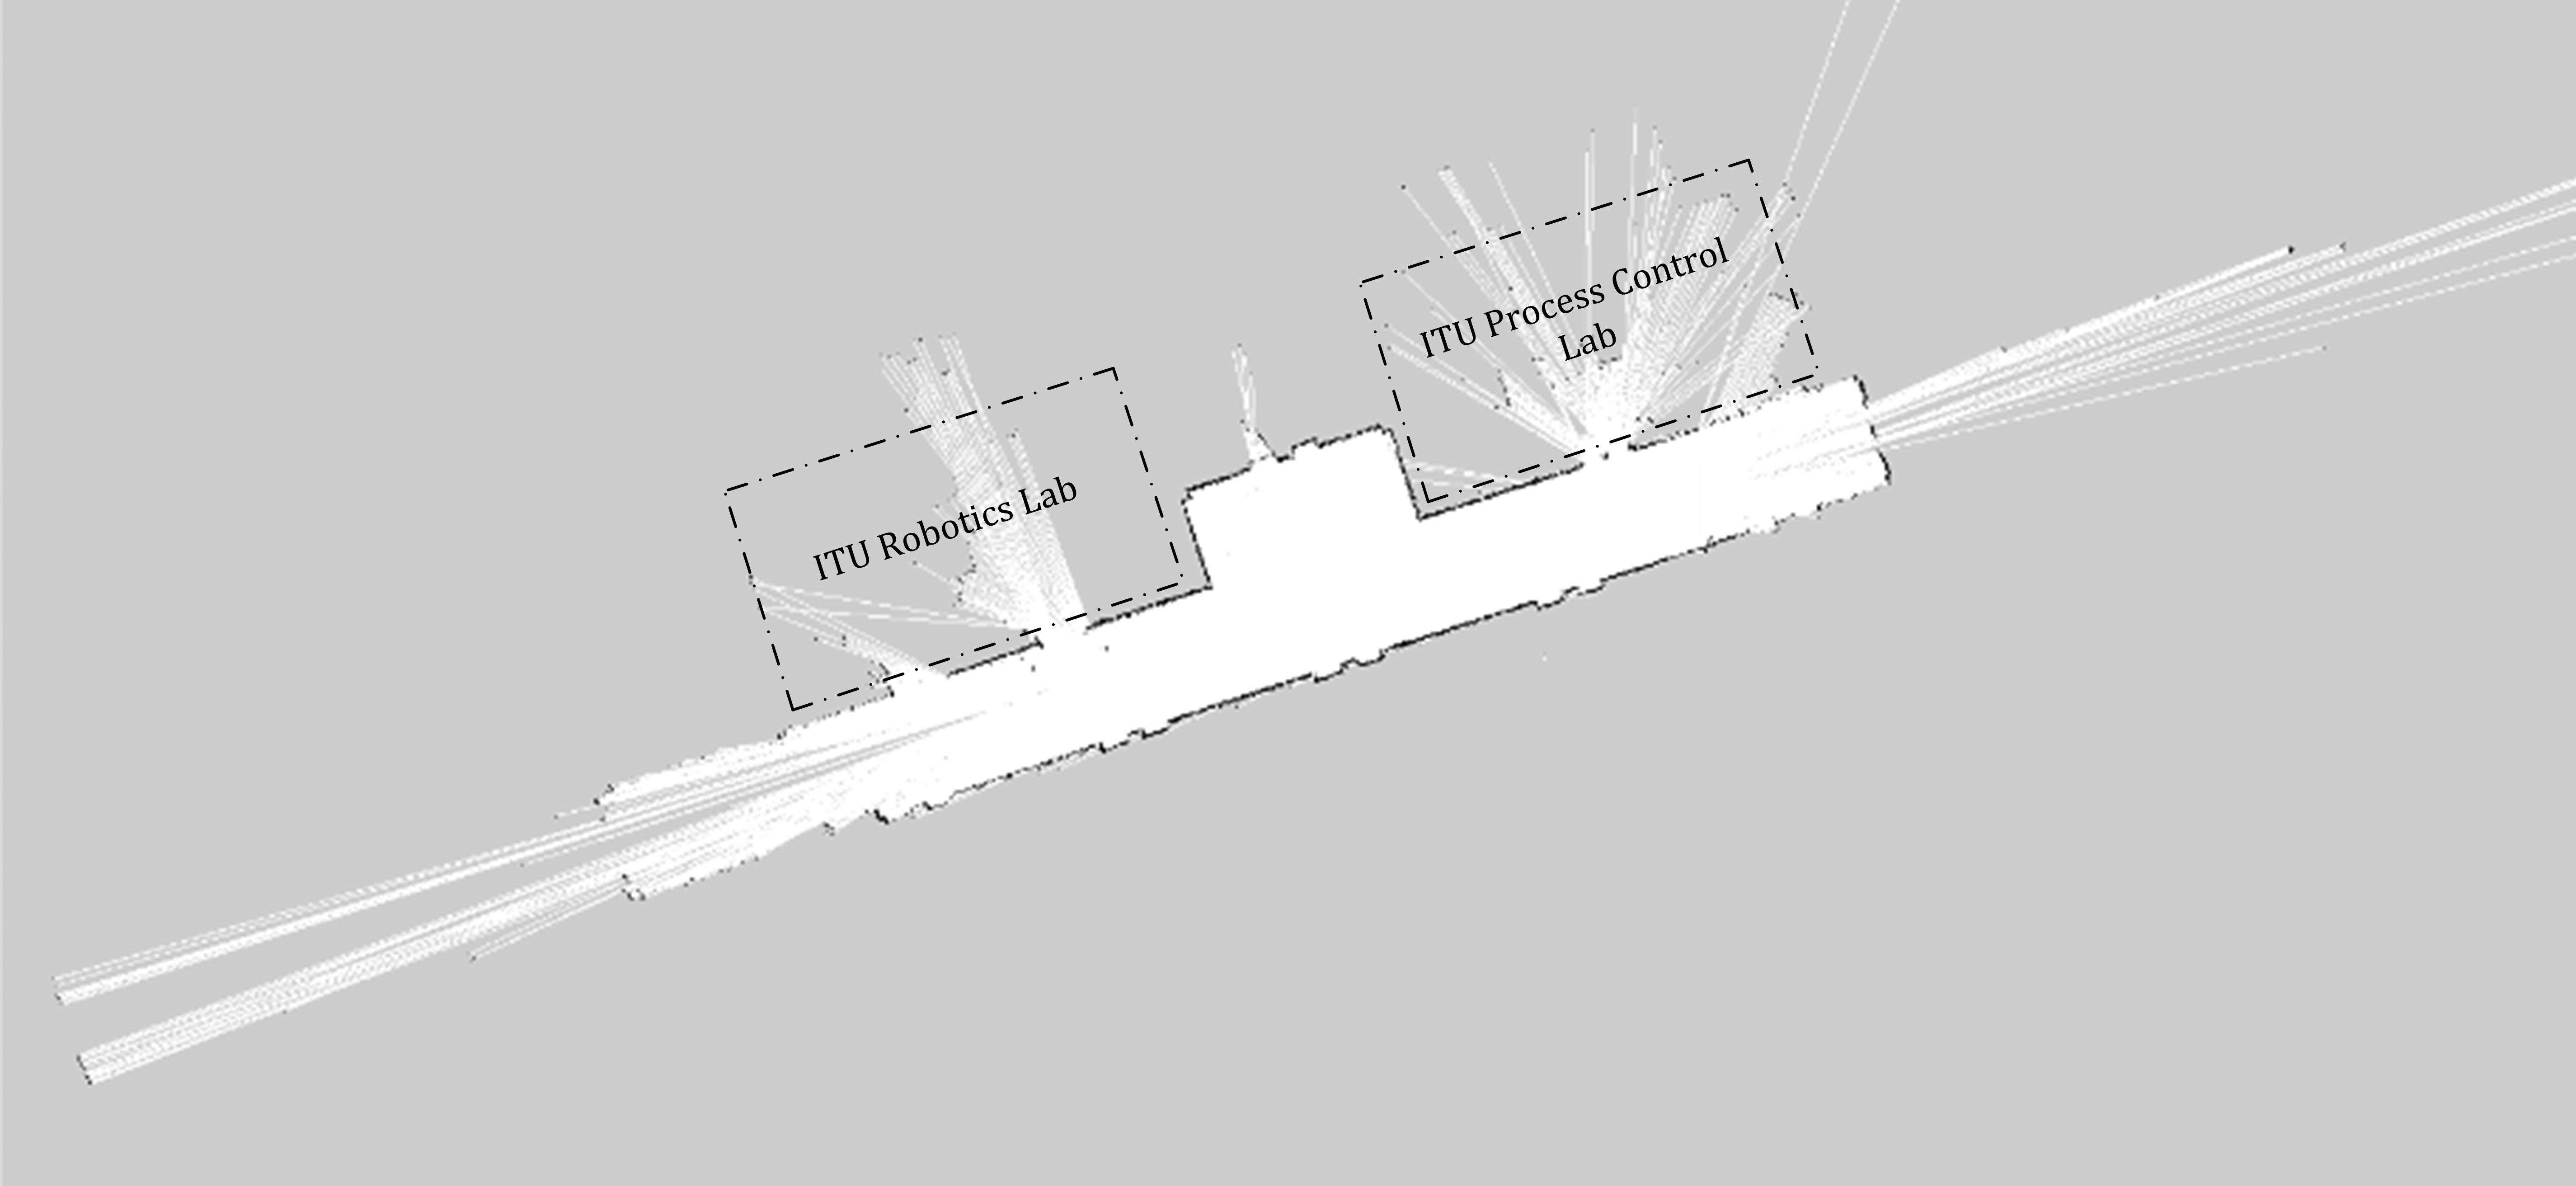
\includegraphics[scale=0.53]{images/map}
		\caption{An offline map of ITU Control and Automation Eng. Department corridor is built with the collected data}
		\label{fig:map}
	\end{figure}				